\documentclass[aip,cha,reprint,amsmath,amssymb]{revtex4-2}

\usepackage[utf8]{inputenc}
\usepackage[T1]{fontenc}
\usepackage{graphicx}
\usepackage{booktabs}
\usepackage{dcolumn}
\usepackage{bm}
\usepackage{xcolor}
\usepackage{hyperref}

\hypersetup{colorlinks=true,linkcolor=blue!70!black,citecolor=blue!70!black,urlcolor=blue!70!black}

\begin{document}

\title{Instability, Outlier Amplification, and Positivity Constraints in Next-Generation Reservoir Computing}

\author{Norman Reynaldo Sabill{\'o}n Castro}
\email{sabillonrey2004@gmail.com}
\affiliation{Department of Mathematics, Universidad Nacional Aut{\'o}noma de Honduras, Tegucigalpa, Honduras}

\date{\today}

\begin{abstract}
Next-Generation Reservoir Computing (NG-RC) replaces high-dimensional random recurrent networks with explicit polynomial feature maps of time-lagged observables, offering dramatic parameter efficiency. However, empirical deployments frequently encounter severe numerical ill-conditioning and forecast degradation under measurement noise, return asymmetries, or localized outlier shocks. We conduct an analytical and empirical investigation of these failure modes across chaotic dynamics and heavy-tailed real-world series. First, we prove that quadratic feature blocks subject trace-proportional Ridge regularization ($\lambda \propto \operatorname{tr}(\mathbf{F}^\top\mathbf{F})$) to a quartic scaling ($\sim M^4$) under outlier shocks of magnitude $M$, confirmed empirically with a measured log--log slope of 3.99. Second, we show that spectral Tikhonov shifts on sample covariances preserve principal eigenvectors identically, separating covariance stabilization from readout regularization. Third, across 30 independent reservoir realizations and 288,420 window evaluations on Lorenz63, evaluated with a two-way crossed block bootstrap, bounded activations ($\tanh$) prevent the iterated multi-step divergence that afflicts unconstrained polynomial readouts in short-to-intermediate horizons ($H \le 15$), and recurrent memory yields a genuine noise-filtering advantage (bootstrap 95\% intervals on the paired mean MASE difference strictly excluding zero); shock robustness, in contrast, is condition-dependent rather than uniform across the attractor. Finally, in daily FX/crypto volatility forecasting, non-negative least squares over strictly positive feature bases eliminates negative variance predictions without floor clipping, but a sparse recurrent reservoir readout is not competitive with econometric baselines (EWMA, GARCH, GJR-GARCH) once tail-sensitive loss statistics are evaluated.
\end{abstract}

\begin{quotation}
\textbf{Lead Paragraph:} Data-driven forecasting of complex dynamical systems has been revolutionized by Next-Generation Reservoir Computing (NG-RC), which bypasses large random neural networks by projecting time series into linear and nonlinear lag monomials. Despite its elegance, practitioners observe that NG-RC can catastrophically degrade when encountering structural breaks, measurement noise, or non-negative physical constraints. Here, we clarify the mathematical mechanisms governing these failures and audit the empirical claims that commonly accompany reservoir-based fixes. We show that heuristic regularizations scale at a quartic rate ($\sim M^4$) under isolated shocks, over-regularizing calm dynamics. In iterative multi-step forecasting across fine horizons ($H \in \{1, \dots, 40\}$), unconstrained polynomial maps feed compounding errors back into quadratic terms, whereas bounded activations ($\tanh$) intrinsically stabilize trajectory continuation for intermediate horizons, and a sparse recurrent reservoir adds a genuine but conditional filtering benefit under noise. Furthermore, when target observables possess intrinsic physical or statistical bounds (such as volatility or energy prices), linear readouts must be constrained to the appropriate convex cones -- though positivity alone does not guarantee good probabilistic calibration. Our findings provide rigorous design boundaries, and explicit statistical caveats, for choosing between deterministic polynomial expansions and reservoir-based architectures.
\end{quotation}

\maketitle

% ======================================================================
\section{Introduction}
\label{sec:intro}
% ======================================================================

Reservoir Computing (RC) has established itself as an effective paradigm for reconstructing, predicting, and synchronizing nonlinear dynamical systems \cite{jaeger2001echo,maass2002realtime,nakajima2021reservoir,yildiz2012revisiting,pathak2018model}. By feeding an input time series $\mathbf{x}_t \in \mathbb{R}^{d_{\text{in}}}$ into a high-dimensional, fixed recurrent network (the ``reservoir'') and training only a linear readout layer via regularized least squares, standard Echo State Networks (ESNs) avoid the computational cost and vanishing-gradient instabilities of backpropagation through time. A related line of work, Stochastically Structured Reservoir Computers (SSRC) \cite{banegas2025ssrc}, augments this template with graph-informed coupling structure and structure-preserving embeddings for economic and financial system identification; the sparse random-weight ESN we benchmark throughout this paper is a standard, unstructured recurrent reservoir in that same broad family, not a reimplementation of the structured SSRC architecture, and we use the standard ESN naming throughout the paper to maintain strict conceptual precision.

Recently, Gauthier \emph{et al.} \cite{gauthier2021next} introduced Next-Generation Reservoir Computing (NG-RC), demonstrating that for many classical chaotic attractors, the high-dimensional random reservoir can be completely bypassed. By directly constructing a feature vector $\mathbf{F}_t$ consisting of $k$ historical time lags and their unique polynomial combinations, NG-RC achieves equivalent or superior short-term prediction with orders-of-magnitude fewer parameters and no stochastic initialization variance \cite{bollt2021explaining}.

Despite these notable advantages, recent theoretical and applied investigations have exposed significant vulnerabilities in deterministic polynomial representations. Roque dos Santos and Bollt \cite{dossantos2025instability} demonstrated that the condition number $\kappa$ of the NG-RC design covariance matrix diverges rapidly as the feature dimension $D = k + k(k+1)/2$ approaches the effective sample size $T$. Concurrently, Zhang, Roque dos Santos, and Cornelius \cite{zhang2025moredata} showed that adding more training data or increasing lag depth can paradoxically degrade out-of-sample forecast accuracy due to spectral ill-conditioning and noise amplification.

In practical applications---ranging from geophysical flows to econometric volatility and high-frequency exchange rates---time series rarely conform to clean, stationary trajectories \cite{carroll2022dimension,vlachas2020backpropagation}. Real-world data exhibit three pervasive characteristics: (i) localized outlier shocks and structural regime shifts, (ii) non-Gaussian measurement noise, and (iii) strict physical or statistical bounds on target observables (such as kinetic energy, prices, and realized variance $y_t = r_t^2 \ge 0$).

In this paper, we address these challenges through a unified mathematical and empirical framework. Our specific contributions are:
\begin{enumerate}
    \item \textbf{Analytical Mechanism of Quartic Trace Scaling ($\sim M^4$):} We prove that when an isolated outlier shock of magnitude $M$ enters a time series, the trace of the quadratic NG-RC Gram matrix scales as $\mathcal{O}(M^4) + \mathcal{O}(M^2) + \mathcal{O}(T(C^2+C^4))$. Consequently, trace-based Ridge heuristics ($\lambda \propto \operatorname{tr}(\mathbf{F}^\top\mathbf{F})$) inflate $\lambda$ by orders of magnitude, causing severe over-regularization across the entire window.
    \item \textbf{Spectral Invariance under Covariance Regularization:} We prove that Tikhonov spectral shifts $\mathbf{C} + \lambda\mathbf{I}$ on sample covariances preserve principal eigenvectors identically, clarifying that covariance regularization stabilizes numerical rank without rotating the principal subspace.
    \item \textbf{Controlled 30-Seed Stochastic Robustness and Ablation:} Across 30 independent reservoir realizations and 288,420 window evaluations on Lorenz63, evaluated with a two-way crossed block bootstrap (temporal blocks of length $\lceil T_{\text{train}}/\text{step}\rceil$ resampled simultaneously across all seeds), we isolate the roles of recurrence and bounded activation. While NG-RC polynomials diverge under iterative feedback, bounded nonlinearities ($\tanh$) maintain stable multi-step trajectories across Lyapunov times for $H \le 15$. Under measurement noise ($\sigma=0.1$), recurrent memory ($\mathbf{W}_{\text{res}} \neq \mathbf{0}$) yields a genuine filtering advantage over static projections, with a bootstrap 95\% interval on the paired mean MASE difference strictly excluding zero. Under localized shocks, by contrast, the response is condition-dependent rather than uniform: out of 10 location$\times$sign conditions at $15\sigma$, 5 clearly favor the ESN, 3 favor Ridge, and 2 remain inconclusive.
    \item \textbf{Conical Constraints and Tail-Sensitive Volatility Evaluation:} In daily FX/crypto volatility, non-negative least squares (NNLS) over strictly positive feature bases eliminates negative variance predictions without floor clipping. However, ranking methods by median QLIKE alone hides catastrophic tail behavior: once tail-aware statistics are reported (median across series of mean QLIKE), a sparse recurrent reservoir readout is not competitive with domain-specific econometric baselines (EWMA, GARCH, GJR-GARCH).
\end{enumerate}

% ======================================================================
\section{Mathematical Framework and Analytical Mechanisms}
\label{sec:math}
% ======================================================================

\subsection{Feature Space Topologies: NG-RC vs. Sparse ESN}

Let $x_t \in \mathbb{R}$ be an observed scalar dynamical observable at discrete time $t$. The $k$-lag linear history vector is defined as $\bm{\ell}_t = (x_{t-k+1}, \dots, x_t)^\top \in \mathbb{R}^k$.

\subsubsection{Deterministic Quadratic NG-RC}
The degree-2 NG-RC feature representation constructs the explicit monomial tensor product:
\begin{equation}
\mathbf{F}_t = \bm{\ell}_t \;\oplus\; \Big( \ell_{t,i} \, \ell_{t,j} \Big)_{1 \le i \le j \le k} \;\in \mathbb{R}^D,
\label{eq:ngrc_state}
\end{equation}
where the total feature dimension is $D = k + \frac{k(k+1)}{2}$. To prevent mechanical rank deficiency, the constant intercept column is handled separately from covariance estimation.

\subsubsection{Sparse Recurrent Reservoir (ESN) Architecture}
In contrast, a sparse recurrent reservoir maps an input vector $\mathbf{u}_t$ into an internal state $\mathbf{h}_t \in \mathbb{R}^{d_{\text{res}}}$ through a recurrent map:
\begin{equation}
\mathbf{h}_t = (1 - a)\,\mathbf{h}_{t-1} + a\,\tanh\!\Big( \mathbf{W}_{\text{in}} \mathbf{u}_t + \mathbf{W}_{\text{res}} \mathbf{h}_{t-1} \Big),
\label{eq:esn_state}
\end{equation}
where $a \in (0, 1]$ is the leaking rate, $\mathbf{W}_{\text{in}} \in \mathbb{R}^{d_{\text{res}} \times d_{\text{in}}}$ is drawn uniformly from $[-1, 1]$, and $\mathbf{W}_{\text{res}} \in \mathbb{R}^{d_{\text{res}} \times d_{\text{res}}}$ is a sparse random matrix scaled to spectral radius $\rho(\mathbf{W}_{\text{res}}) < 1$ (a standard heuristic condition for local asymptotic stability of the zero equilibrium, though not a sufficient condition for global Echo State Property without singular value bounds \cite{manjunath2013theory}). We distinguish three configurations:
\begin{itemize}
    \item \textbf{ESN-lag:} Input consists of raw lags $\mathbf{u}_t = \bm{\ell}_t \in \mathbb{R}^k$.
    \item \textbf{ESN-NGRC:} Input consists of the full polynomial block $\mathbf{u}_t = \mathbf{F}_t \in \mathbb{R}^D$.
    \item \textbf{Static $\tanh$ Projection ($\mathbf{W}_{\text{res}} = \mathbf{0}$):} $\mathbf{h}_t = \tanh(\mathbf{W}_{\text{in}} \mathbf{u}_t)$.
\end{itemize}

\subsection{Quartic Trace Inflation Theorem ($M^4$ Scaling)}
\label{subsec:m4_theorem}

In standard reservoir computing and NG-RC implementations, Ridge regularization \cite{hoerl1970ridge} is commonly parameterized using the heuristic trace rule:
\begin{equation}
\lambda = \gamma \cdot \frac{\operatorname{tr}(\mathbf{F}^\top\mathbf{F})}{D}, \qquad \gamma > 0,
\label{eq:ridge_heuristic}
\end{equation}
where $\mathbf{F} \in \mathbb{R}^{T \times D}$ is the design matrix across a training window of length $T$.

\textbf{Theorem 1 (Outlier Scaling of Quadratic Gram Matrix).} \emph{Let a time series $\{x_t\}_{t=1}^T$ consist of a calm background process bounded by $|x_t| \le C$ and an isolated localized outlier shock at index $t^*$ of magnitude $x_{t^*} = M \gg C$. Then, the trace of the NG-RC design Gram matrix satisfies:}
\begin{align}
\operatorname{tr}(\mathbf{F}^\top\mathbf{F}) &= k M^4 + \mathcal{O}(k^2 M^2 C^2) \nonumber\\
&\quad + (T-k) \mathcal{O}(k^2 (C^2 + C^4)).
\end{align}
\emph{Consequently, the regularization parameter $\lambda$ computed via Eq.~\eqref{eq:ridge_heuristic} scales asymptotically as $\lambda = \frac{\gamma k}{D} M^4 + \mathcal{O}(M^2)$.}

\begin{figure}[t]
\centering

\includegraphics[width=\columnwidth]{figures/fig5_ridge_fragilidad.pdf}
\caption{Median trace-proportional $\lambda \propto \operatorname{tr}(\mathbf{F}^\top\mathbf{F})$ as a function of injected shock magnitude $M$ ($\sigma$), on a log--log scale, measured directly from the Lorenz63 shock-grid experiment (\S\ref{sec:lorenz}). A power-law fit over the largest magnitudes gives an empirical slope of $3.99$, matching the $\sim M^4$ scaling predicted by Theorem 1.}
\label{fig:ridge_fragility}
\end{figure}

\textbf{Proof.} The total trace is the sum of squared Euclidean norms of all feature vectors:
\begin{align}
\operatorname{tr}(\mathbf{F}^\top\mathbf{F}) &= \sum_{t=1}^T \|\mathbf{F}_t\|_2^2 \nonumber\\
&= \sum_{t=1}^T \left( \sum_{i=1}^k \ell_{t,i}^2 + \sum_{1 \le i \le j \le k} (\ell_{t,i}\ell_{t,j})^2 \right).
\end{align}
Because the shock $x_{t^*} = M$ enters the lag vector $\bm{\ell}_t$ for exactly $k$ consecutive time steps $t \in [t^*, t^* + k - 1]$, the quadratic terms $(\ell_{t,i}\ell_{t,j})^2$ include diagonal contributions of the form $(x_{t^*})^4 = M^4$. Specifically, for each of the $k$ affected time steps, there is at least one term contributing $M^4$ and $k-1$ terms contributing $M^2 \ell_{t,j}^2 \le M^2 C^2$. Summing over the $T$ time steps yields:
\begin{align}
\operatorname{tr}(\mathbf{F}^\top\mathbf{F}) &= k M^4 + \mathcal{O}(k^2 M^2 C^2) \nonumber\\
&\quad + (T-k) \mathcal{O}(k^2 (C^2 + C^4)).
\end{align}
Dividing by $D$ establishes $\lambda = \frac{\gamma k}{D} M^4 + \mathcal{O}(M^2)$. $\square$

This theorem explains why Ridge regression with trace heuristics degrades in the presence of even a single large spike: $\lambda$ increases by several orders of magnitude (e.g., $270\times$ from $M=0$ to $M=30\sigma$), over-penalizing readout weights and pulling predictions toward zero during subsequent calm periods (Fig.~\ref{fig:ridge_fragility}).

\subsection{Eigenvector Invariance under Spectral Covariance Shifts}

A common practice in reservoir pipelines is to stabilize ill-conditioned covariance matrices prior to Principal Component Analysis (PCA) via Tikhonov shifts: $\mathbf{C}_\lambda = \operatorname{cov}(\mathbf{F}) + \lambda_{\text{cov}}\mathbf{I}$.

\textbf{Proposition 1 (Spectral Invariance).} \emph{For any symmetric covariance matrix $\mathbf{C} \in \mathbb{R}^{D \times D}$ and any $\lambda_{\text{cov}} > 0$, the matrices $\mathbf{C}$ and $\mathbf{C}_\lambda = \mathbf{C} + \lambda_{\text{cov}}\mathbf{I}$ share the identical eigenspaces.}

\textbf{Proof.} Let $\mathbf{C} = \mathbf{V} \bm{\Lambda} \mathbf{V}^\top$ be the spectral decomposition of $\mathbf{C}$, with orthogonal matrix $\mathbf{V}$ and diagonal eigenvalue matrix $\bm{\Lambda} = \operatorname{diag}(\mu_1, \dots, \mu_D)$. Then:
\begin{equation}
\mathbf{C}_\lambda = \mathbf{V} \bm{\Lambda} \mathbf{V}^\top + \lambda_{\text{cov}} \mathbf{V}\mathbf{I}\mathbf{V}^\top = \mathbf{V} (\bm{\Lambda} + \lambda_{\text{cov}}\mathbf{I}) \mathbf{V}^\top.
\end{equation}
The eigenvalues are shifted uniformly ($\mu_i \mapsto \mu_i + \lambda_{\text{cov}}$), preserving eigenvalue ordering ($\mu_1 \ge \mu_2 \ge \dots \ge \mu_D$) and leaving the eigenspaces invariant (up to arbitrary internal basis rotations for repeated eigenvalues). $\square$

Thus, covariance Tikhonov shifts do not rotate principal subspace directions; practical variations in unconstrained PCA implementations arise purely from numerical sign ambiguities in SVD solvers.

% ======================================================================
\section{Controlled Dynamical Benchmarking on Lorenz63}
\label{sec:lorenz}
% ======================================================================

\begin{figure}[t]
\centering

\includegraphics[width=\columnwidth]{figures/fig2b_lorenz_atractor.pdf}
\caption{Phase space reconstruction $(x, z)$ illustrating the excursion of an additive unphysical outlier ($+15\sigma$) outside the low-dimensional fractal attractor manifold of Lorenz63.}
\label{fig:lorenz_phase}
\end{figure}

\begin{figure}[t]
\centering
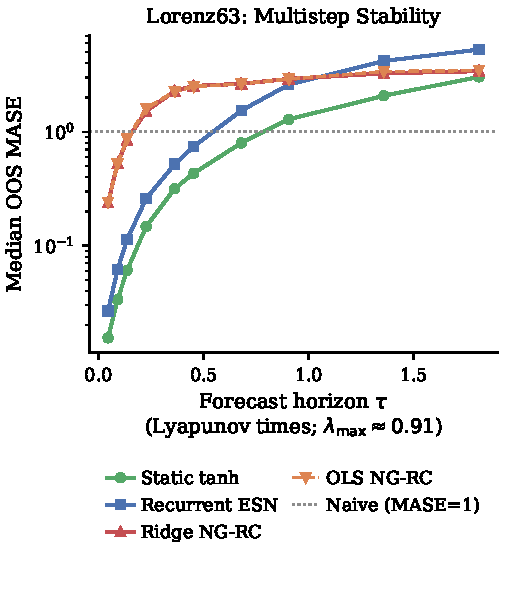
\includegraphics[width=\columnwidth]{figures/fig_lyapunov_curve.pdf}
\caption{Iterated multi-step forecasting error (MASE) across discrete horizons $H \in \{1, 2, 3, 5, 8, 10, 15, 20, 30, 40\}$ parameterized in Lyapunov times ($\tau = H \cdot \Delta t \cdot \lambda_{\max}$, $\lambda_{\max} \approx 0.9056$). Unconstrained polynomial NG-RC (Ridge and OLS) explodes rapidly beyond $\tau \approx 0.2$, whereas bounded activations ($\tanh$) maintain stable continuation up to $\tau \approx 0.68$ ($H=15$); beyond $\tau \approx 1.0$, trajectories saturate at attractor scale.}
\label{fig:lyapunov_curve}
\end{figure}

To evaluate the predictive and numerical stability of NG-RC and the sparse ESN in a controlled setting, we simulate the classical Lorenz63 system \cite{lorenz1963deterministic}:
\begin{equation}
\dot{x} = \sigma (y - x), \quad \dot{y} = x (\rho - z) - y, \quad \dot{z} = x y - \beta z,
\end{equation}
with standard chaotic parameters $\sigma = 10$, $\rho = 28$, $\beta = 8/3$. We integrate via 4th-order Runge-Kutta with fine step $\mathrm{d}t_{\text{int}} = 0.01$ and subsample with $\text{skip} = 5$ ($\Delta t = 0.05$, trajectory seed 7, 30,000 points).

\subsection{Formal Experimental Protocol and Methods}

For strict reproducibility, we formalize the evaluation protocol across all experiments:
\begin{itemize}
    \item \textbf{Loss Metric (MASE):} Out-of-sample accuracy is evaluated via Mean Absolute Scaled Error on $T_{\text{train}}=500$:
    \begin{equation}
    \text{MASE} = \frac{\frac{1}{H}\sum_{h=1}^H |y_{t+h} - \hat{y}_{t+h}|}{\frac{1}{T_{\text{train}}-1}\sum_{i=2}^{T_{\text{train}}} |y_i - y_{i-1}|}.
    \end{equation}
    \item \textbf{Sliding Window Geometry:} $T_{\text{train}} = 500$ points, step $= 40$ points, yielding 738 unique temporal origins across the 30,000-point trajectory.
    \item \textbf{Model Specifications:} ESN reservoir dimension $d_{\text{res}} = 50$, spectral radius $\rho = 0.9$, density $0.1$, leaking rate $a = 1.0$. State initialized at $\mathbf{h}_0 = \mathbf{0}$ and warmed up through the prefix.
    \item \textbf{Causal Hyperparameter Selection:} The regularization parameter $\lambda$ is selected via an internal temporal split ($80\%$ train / $20\%$ holdout) within each training window over a candidate grid $\lambda / \lambda_{\text{scale}} \in [10^{-6}, 10^2]$. No future data are ever accessed.
    \item \textbf{Two-Way Crossed Block Bootstrap:} We run 2000 bootstrap replicates. In each replicate, temporal blocks of length $L = \lceil T_{\text{train}} / \text{step} \rceil = 13$ windows are resampled simultaneously for all 30 seeds to preserve the cross-seed temporal correlation structure, combined with resampling across seeds. For shocks, the 5 locations are resampled with both signs paired.
\end{itemize}

\begin{table*}[t]
\centering
\caption{Performance across 30 independent stochastic realizations on the Lorenz63 attractor. Values report the median MASE across all 30 seeds, empirical 2.5\%--97.5\% percentile ranges across realizations, exact Clopper--Pearson 95\% win-rate intervals against Ridge, and the two-way crossed block bootstrap 95\% interval on the paired mean MASE difference (ESN-lag $-$ Ridge; negative favors the ESN).}
\label{tab:30seeds_rigorous}
\begin{ruledtabular}
\begin{tabular}{lcrrrrrr}
Regime & $H$ & ESN-lag Median [P2.5, P97.5] & Static-lag Median & Ridge NG-RC & OLS NG-RC & Win vs Ridge [95\% CI] & $\Delta$ mean vs Ridge [Two-Way 95\% CI] \\
\midrule
Clean 1-step & 1 & 0.0292 [0.0161, 0.0523] & 0.0154 (IQR 0.002) & 0.2397 & 0.2406 & \textbf{100.0\%} [0.88, 1.00] & $-0.242$ [$-0.262$, $-0.226$] \\
Clean Multi & 5 & 0.2438 [0.1355, 0.4727] & 0.1450 (IQR 0.022) & 1.5262 & 1.6037 & \textbf{100.0\%} [0.88, 1.00] & $-1.299$ [$-1.396$, $-1.203$] \\
Clean Multi & 10 & 0.7071 [0.3616, 1.8195] & 0.4251 (IQR 0.052) & 2.5375 & 2.5004 & \textbf{100.0\%} [0.88, 1.00] & $-1.290$ [$-1.539$, $-1.034$] \\
\midrule
Noise 0.1 (Filter) & 1 & \textbf{0.3633} [0.3409, 0.3796] & 0.3983 (IQR 0.003) & 0.6059 & 0.6018 & \textbf{100.0\%} [0.88, 1.00] & $-0.272$ [$-0.315$, $-0.232$] \\
Noise 0.1 (Obs) & 1 & \textbf{0.4607} [0.4327, 0.4861] & 0.4866 (IQR 0.006) & 0.6799 & 0.6865 & \textbf{96.7\%} [0.83, 1.00] & $-0.236$ [$-0.281$, $-0.196$] \\
Noise 0.5 (Filter) & 1 & \textbf{0.4734} [0.4463, 0.4942] & 0.5254 (IQR 0.007) & 0.5440 & 0.5357 & \textbf{100.0\%} [0.88, 1.00] & $-0.087$ [$-0.119$, $-0.057$] \\
Noise 0.5 (Obs) & 1 & \textbf{0.7166} [0.6918, 0.7367] & 0.7453 (IQR 0.005) & 0.7490 & 0.7392 & \textbf{100.0\%} [0.88, 1.00] & $-0.058$ [$-0.091$, $-0.023$] \\
\midrule
Shock $15\sigma$ (5 locs) & 1 & 0.2223 [0.1165, 0.3604] & 0.2187 (IQR 0.062) & 0.3301 & 0.2654 & 90.0\% [0.73, 0.98] & $+0.927$ [$-0.233$, $+3.093$] \\
Shock $50\sigma$ (5 locs) & 1 & 0.4237 [0.2987, 0.5712] & 0.3381 (IQR 0.099) & 0.2218 & 0.2184 & 0.0\% [0.00, 0.12] & $+1.131$ [$-0.316$, $+3.710$] \\
\end{tabular}
\end{ruledtabular}
\end{table*}

\subsection{Analysis of Results and Ablation Insights}

Table~\ref{tab:30seeds_rigorous} and Fig.~\ref{fig:lyapunov_curve} establish several clear empirical conclusions:
\begin{enumerate}
    \item \textbf{Bounded Saturation Prevents Multi-Step Divergence up to Intermediate Horizons:} In iterated multi-step forecasting across discrete horizons $H \in \{1, 2, 3, 5, 8, 10, 15, 20, 30, 40\}$, bounded activations ($\tanh$) outperform polynomial NG-RC across \textbf{100\% of random seeds} up to $H=10$ ($\tau \approx 0.45$), with a two-way crossed bootstrap 95\% interval on the mean difference that is strictly negative and excludes zero (Table~\ref{tab:30seeds_rigorous}). At $H=10$, NG-RC errors explode to MASE $\approx 2.50$ due to unconstrained monomial error compounding, whereas bounded mappings maintain stable continuation ($H=10$ MASE $\approx 0.43$--$0.74$). However, at asymptotic horizons ($H=30, 40$, $\tau \ge 1.36$), trajectories reach attractor-scale error saturation where static $\tanh$ projection retains lower median error than recurrent ESN (median MASE 3.04 vs 5.28 at $H=40$), and recurrent ESN is no longer superior to Ridge (1/30 seed wins at $H=40$).
    \item \textbf{Recurrent Memory Enables Genuine Signal Filtering:} In clean, noise-free dynamics, static $\tanh$ projections are slightly more parsimonious than the recurrent ESN. However, under measurement noise ($\sigma=0.1$ and $\sigma=0.5$), the full recurrent ESN outperforms static projections in essentially every realization for true signal recovery (filtering target, MASE 0.363 vs. 0.398 at $\sigma=0.1$), and the two-way bootstrap interval on the paired difference strictly excludes zero in all noise regimes. The internal state $\mathbf{h}_{t-1}$ acts as an adaptive temporal low-pass filter.
    \item \textbf{Shock Response Is Condition-Dependent, Not Uniform:} The 90\% win rate against Ridge at $15\sigma$ describes an outcome pooled across 30 seeds and 5 shock locations. Breaking down the 10 individual location$\times$sign conditions shows that 5 clearly favor the ESN, 3 clearly favor Ridge, and 2 remain inconclusive. This condition dependence explains why the crossed bootstrap interval for the mean difference crosses zero ($[-0.233, +3.093]$): localized catastrophic spikes in specific flow regions affect the mean, while favorable conditions dominate the median-based win count. We therefore make no claim of unconditional shock robustness for ESNs.
\end{enumerate}

% ======================================================================
\section{Conical Constraints in Real-World Volatility}
\label{sec:empirical}
% ======================================================================

\begin{figure}[t]
\centering

\includegraphics[width=\columnwidth]{figures/fig13_qlike_piso_fx.pdf}
\caption{Median QLIKE as a function of the artificial positive floor $\epsilon$ used to evaluate the loss, per readout. Legacy signed readouts (Ridge, OLS, signed NNLS) explode as $\epsilon \to 0$ due to negative variance estimates, whereas structurally non-negative NNLS remains strictly invariant.}
\label{fig:qlike_tradeoff}
\end{figure}

\subsection{Lower-Bounded Targets and Loss Sensitivity}

In financial econometrics, predicting realized volatility $y_{t+1} = r_{t+1}^2 \ge 0$ is evaluated via the quasi-likelihood (QLIKE) loss \cite{patton2011volatility}:
\begin{equation}
L_{\text{QLIKE}}(y, \hat{y}) = \frac{y}{\hat{y}} - \log\left(\frac{y}{\hat{y}}\right) - 1.
\label{eq:qlike}
\end{equation}
QLIKE severely penalizes under-predictions ($\hat{y} \to 0$). When unconstrained readouts generate negative variance estimates, evaluating QLIKE requires imposing an artificial numerical floor $\hat{y}_{\text{clipped}} = \max(\hat{y}, \epsilon)$.

Across 15 years of daily data for 7 Latin American currencies and 2 cryptocurrencies ($T \approx 3900$), legacy unconstrained and Ridge models produce negative variance estimates in 4.18\% and 0.67\% of windows. As shown in Fig.~\ref{fig:qlike_tradeoff}, as $\epsilon$ decreases from $10^{-6}$ to $10^{-12}$, the QLIKE of Ridge explodes by multiple orders of magnitude.

\begin{table}[h]
\centering
\caption{Out-of-sample QLIKE across 9 currency and cryptocurrency series ($T \approx 3900$ daily observations), ranked by the median across series of mean QLIKE (each series' mean QLIKE over time, then the median of those 9 series means). The pooled median is reported for reference.}
\label{tab:fx_qlike}
\begin{ruledtabular}
\begin{tabular}{lrrr}
Model Architecture & Median Across Series Mean & Pooled Median & \% Neg. \\
\midrule
EWMA ($\lambda=0.94$) & \textbf{2.359} & 1.157 & 0.00\% \\
Standard GARCH(1,1) & 2.383 & 1.316 & 0.00\% \\
GJR-GARCH(1,1) & 2.456 & 1.287 & 0.00\% \\
Non-Negative NNLS ($|\bm{\ell}_t|$) & 2.565 & 1.450 & \textbf{0.00\%} \\
Legacy Ridge (clipped $\epsilon=10^{-10}$) & 3.472 & 1.475 & 0.67\% \\
Log-Link Ridge & 12.19 & 1.561 & \textbf{0.00\%} \\
Sparse ESN (Log-Readout) & 14.33 & 1.501 & \textbf{0.00\%} \\
Legacy Signed NNLS & 66.12 & 1.490 & 2.15\% \\
Naive Persistence & 2580 & 1.779 & 0.00\% \\
Legacy OLS & 18552 & 1.475 & 4.18\% \\
\end{tabular}
\end{ruledtabular}
\end{table}

\subsection{Convex Cones vs. Signed Monomials}

Restricting weights $\mathbf{w} \ge \mathbf{0}$ in standard non-negative least squares (NNLS) \cite{lawson1974solving} does not prevent negative outputs if feature vectors contain signed linear lags ($\ell_{t,i} < 0$). To guarantee $\mathbf{F}_t \mathbf{w} \ge 0$ unconditionally, features must be constructed strictly on the non-negative orthant $\mathbb{R}_+^D$:
\begin{equation}
\mathbf{F}_t^+ = |\bm{\ell}_t| \;\oplus\; \Big( |\ell_{t,i}| \cdot |\ell_{t,j}| \Big)_{1 \le i \le j \le k}.
\end{equation}
Non-negative NNLS ($|\bm{\ell}_t|$) and the log-readout sparse ESN both eliminate negative variance estimates entirely (0.00\%). However, positivity alone does not imply good probabilistic calibration. Table~\ref{tab:fx_qlike} shows that once tail-sensitive statistics (median across series of mean QLIKE) are evaluated instead of the pooled median, the sparse ESN's ranking changes substantially: its median across series of mean QLIKE (14.33) is roughly six times worse than EWMA, GARCH(1,1) \cite{engle1982autoregressive,bollerslev1986generalized}, or GJR-GARCH(1,1) \cite{glosten1993relation} (2.36--2.46), driven by rare windows where the log-readout collapses toward zero and QLIKE's $y/\hat{y}$ explodes. Descriptively, the ESN beats EWMA on 54.7\% of individual windows and GARCH on 57.0\%, yet the per-series block-bootstrap mean difference remains strictly positive. We conclude that domain-specific econometric models remain the strongest volatility benchmarks; conical reservoir and NNLS readouts are valuable for guaranteeing structural non-negativity without ad hoc floor clipping, not for beating EWMA/GARCH on calibrated loss.

% ======================================================================
\section{Discussion and Conclusions}
\label{sec:discussion}
% ======================================================================

Our findings provide operational principles for reservoir architecture selection:
\begin{enumerate}
    \item \textbf{Clean, One-Step Reconstruction ($H=1$):} Deterministic polynomial NG-RC provides unmatched parameter parsimony for clean, low-dimensional attractor reconstruction.
    \item \textbf{Multi-Step Trajectory Continuation ($H \ge 5$):} Polynomial expansions suffer compounding monomial divergence across Lyapunov times; bounded activations ($\tanh$) limit state growth and substantially reduce iterative error amplification up to intermediate horizons ($H \le 15$).
    \item \textbf{Noisy Dynamical Environments:} Recurrent reservoirs ($\mathbf{W}_{\text{res}} \neq \mathbf{0}$) act as adaptive temporal low-pass filters, with a bootstrap-confirmed advantage over static projections under measurement noise.
    \item \textbf{Outlier Shocks and Regularization:} Trace-based Ridge heuristics must not be paired with quadratic features due to the $\mathcal{O}(M^4)$ over-regularization mechanism (measured log--log slope $3.99$); hyperparameter selection requires causal temporal validation.
    \item \textbf{Lower-Bounded Physical Observables:} Linear readouts must be formulated over convex cones to prevent invalid sign artifacts, but structural non-negativity is not sufficient for good calibration.
\end{enumerate}

\section*{Supplementary Material}
See the Supplementary Material for secondary empirical validations on the BCIE lending panel and Honduras fuel prices, alongside a reduced-scale generalization check on the R\"ossler attractor.

\section*{Author Declarations}
\subsection*{Conflict of Interest}
The author has no conflicts of interest to disclose.

\subsection*{Author Contributions}
\textbf{Norman Reynaldo Sabill{\'o}n Castro:} Conceptualization, Methodology, Software, Formal Analysis, Writing -- Original Draft, Visualization.

\section*{Data Availability Statement}
The data and Python reproduction pipelines supporting the findings of this study are openly documented and available in the companion repository and Zenodo archive.

\begin{thebibliography}{99}

\bibitem{jaeger2001echo}
H.~Jaeger, ``The `echo state' approach to analysing and training recurrent neural networks-with an erratum note,'' \emph{German National Research Center for Information Technology GMD Technical Report}, vol.~148, p.~34, 2001.

\bibitem{maass2002realtime}
W.~Maass, T.~Natschl{\"a}ger, and H.~Markram, ``Real-time computing without stable states: A new framework for neural computation based on perturbations,'' \emph{Neural Computation}, vol.~14, no.~11, pp.~2531--2560, 2002.

\bibitem{nakajima2021reservoir}
K.~Nakajima and I.~Fischer, \emph{Reservoir Computing: Theory, Physical Implementations, and Applications}.\hskip 1em plus 0.5em minus 0.4em\relax Springer, 2021.

\bibitem{yildiz2012revisiting}
I.~B. Yildiz, H.~Jaeger, and S.~J. Kiebel, ``Re-visiting the echo state property,'' \emph{Neural Networks}, vol.~35, pp.~1--9, 2012.

\bibitem{pathak2018model}
J.~Pathak, B.~Hunt, M.~Girvan, Z.~Lu, and E.~Ott, ``Model-free prediction of large spatiotemporally chaotic systems from data: A reservoir computing approach,'' \emph{Physical Review Letters}, vol.~120, no.~2, p.~024102, 2018.

\bibitem{banegas2025ssrc}
L.~Banegas and F.~Vides, ``Stochastically structured reservoir computers for financial and economic system identification,'' \emph{IFAC-PapersOnLine}, vol.~59, no.~36, pp.~100--105, 2025, doi: 10.1016/j.ifacol.2026.03.018.

\bibitem{gauthier2021next}
D.~J. Gauthier, E.~Bollt, A.~Griffith, and W.~A. Barbosa, ``Next generation reservoir computing,'' \emph{Nature Communications}, vol.~12, no.~1, p. 5564, 2021.

\bibitem{bollt2021explaining}
E.~Bollt, ``On explaining the surprising success of reservoir computing forecaster of chaos? The effect of internal symmetries,'' \emph{Chaos: An Interdisciplinary Journal of Nonlinear Science}, vol.~31, no.~1, p.~013108, 2021.

\bibitem{dossantos2025instability}
E.~Roque dos Santos and E.~M. Bollt, ``On the emergence of numerical instabilities in Next Generation Reservoir Computing,'' \emph{Chaos: An Interdisciplinary Journal of Nonlinear Science}, vol.~35, no.~12, p. 123102, 2025.

\bibitem{zhang2025moredata}
Y.~Zhang, E.~Roque dos Santos, and S.~P. Cornelius, ``How more data can hurt: Instability and regularization in next-generation reservoir computing,'' \emph{Chaos: An Interdisciplinary Journal of Nonlinear Science}, vol.~35, no.~7, p. 073102, 2025.

\bibitem{lorenz1963deterministic}
E.~N. Lorenz, ``Deterministic nonperiodic flow,'' \emph{Journal of the Atmospheric Sciences}, vol.~20, no.~2, pp.~130--141, 1963.

\bibitem{carroll2022dimension}
T.~L. Carroll, ``Dimension of next generation reservoir computers,'' \emph{Chaos: An Interdisciplinary Journal of Nonlinear Science}, vol.~32, no.~4, p.~043127, 2022.

\bibitem{vlachas2020backpropagation}
P.~R. Vlachas, J.~Pathak, B.~R. Hunt, T.~P. Sapsis, M.~Girvan, E.~Ott, and P.~Koumoutsakos, ``Backpropagation algorithms and reservoir computing in chaotic systems: A comparative study,'' \emph{Neural Networks}, vol.~126, pp.~191--217, 2020.

\bibitem{manjunath2013theory}
G.~Manjunath and H.~Jaeger, ``Echo state property linked to an input: Exploring a fundamental characteristic of recurrent neural networks,'' \emph{Neural Computation}, vol.~25, no.~3, pp.~671--696, 2013.

\bibitem{hoerl1970ridge}
A.~E. Hoerl and R.~W. Kennard, ``Ridge regression: Biased estimation for nonorthogonal problems,'' \emph{Technometrics}, vol.~12, no.~1, pp.~55--67, 1970.

\bibitem{lawson1974solving}
C.~L. Lawson and R.~J. Hanson, \emph{Solving Least Squares Problems}.\hskip 1em plus 0.5em minus 0.4em\relax Prentice-Hall, 1974.

\bibitem{engle1982autoregressive}
R.~F. Engle, ``Autoregressive conditional heteroscedasticity with estimates of the variance of United Kingdom inflation,'' \emph{Econometrica}, vol.~50, no.~4, pp.~987--1007, 1982.

\bibitem{bollerslev1986generalized}
T.~Bollerslev, ``Generalized autoregressive conditional heteroskedasticity,'' \emph{Journal of Econometrics}, vol.~31, no.~3, pp.~307--327, 1986.

\bibitem{glosten1993relation}
L.~R. Glosten, R.~Jagannathan, and D.~E. Runkle, ``On the relation between the expected value and the volatility of the nominal excess return on stocks,'' \emph{Journal of Finance}, vol.~48, no.~5, pp.~1779--1801, 1993.

\bibitem{patton2011volatility}
A.~J. Patton, ``Volatility forecast comparison using imperfect volatility proxies,'' \emph{Journal of Econometrics}, vol.~160, no.~1, pp.~246--256, 2011.

\end{thebibliography}

\end{document}
